\begin{figure}
\begin{center}
    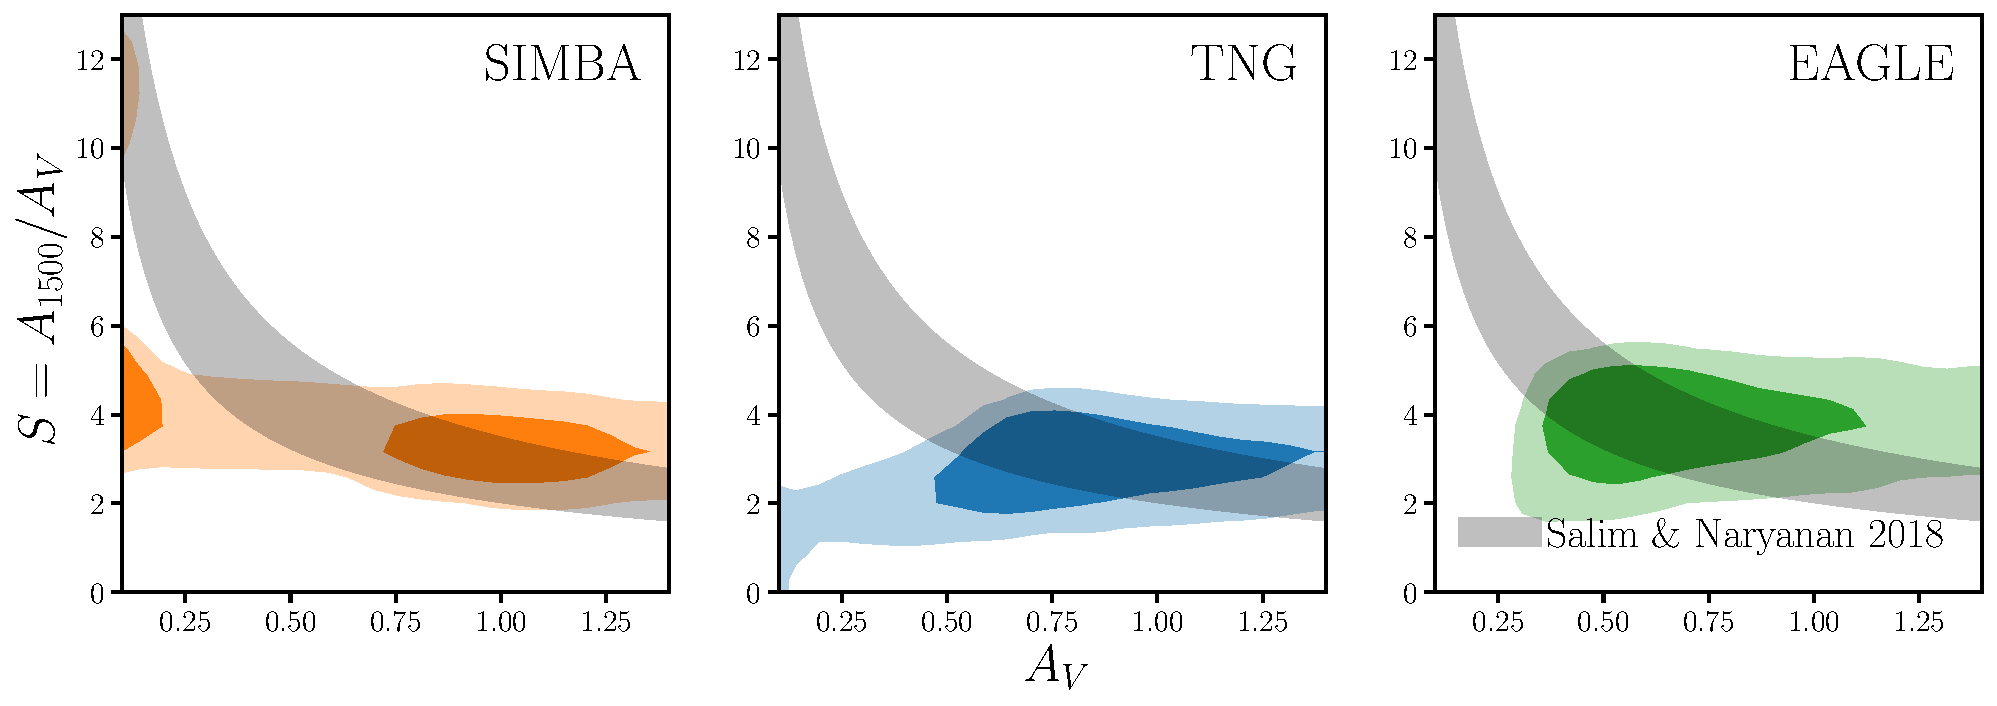
\includegraphics[width=0.4\textwidth]{figs/abc_slope_AV_all.pdf}
    \caption{\label{fig:slope}
    The attenuation-slope relation of the attenuation curves predicted by our  
    \eda~prescription for the median posterior parameter values of TNG (blue) and EAGLE
    (green). For comparison, we include the observed attenuation-slope relation
    from GSWLC2~\citep{salim2020}. We also include the Milky Way (star) and
    mark the slope of the \cite{calzetti2001} curve (dashed). We use $A_V$ and
    $S = A(1500\AA)/A_V$ as measurements of attenuation and slope, respectively. 
    We derived the posteriors of the \eda~parameters from comparing the
    UV and optical color-magnitude relation and do not fit any observed dust
    attenuation measurements. Yet, \emph{we find excellent agreement between
    the attenuation-slope relation predicted by the \eda~and observations.}
    }
\end{center}
\end{figure}

\subsection{Reproducing Dust Observations} 
\chedit{
    With our \eda~prescription, we are able to accurately reproduce the
    observed optical and UV color-magnitude relations with our simulations. 
    In addition to  reproducing observations, since the \eda~assigns dust
    attenuation curves for each simulated galaxies, we can also compare the
    \eda~dust attenuation curves to dust attenuation measured from
    observations. 
    We begin with the well-established attenuation-slope relation: galaxies
    with higher dust attenuations have shallower attenuation curves. 
    This relation is a consequence of dust scattering dominating absoprtion at
    low attenuation while dust absorption dominating at high
    attenuation~\citep{gordon1994, witt2000, draine2003, chevallard2013}. 
}
In Figure~\ref{fig:slope}, we present the attenuation-slope relation of the
dust attenuation curves predicted by the \eda~for the median posteriors of TNG
(blue) and EAGLE (green).
\chedit{
    For comparison, we include the observed attenuation-slope relations of
    GSWLC2 galaxies~\citep[grey shaded;][]{salim2020}, the Milky Way (star),
    and mark the slope of the \cite{calzetti2001} curve (dashed).
    For attenuation we use $A_V$ and for slope we use the UV-optical slope, $S
    = A(1500\AA)/A_V$, commonly found in the literature. The contours mark the 68
    and 95 percentiles. 
    We note that the different in the $A_V$ ranges is due to the $M_r$
    completeness limit imposed by our forward model (Section~\ref{sec:fm}).
    The GSWLC2 sample in \cite{salim2020} extends down to $M_* \sim
    10^{8.5}M_\odot$; however, the TNG and EAGLE samples do not extend below
    $M_* \sim10^{10}M_\odot$.
    \emph{The \eda~predicts attenuation-slope relations for TNG and EAGLE that
    are in excellent agreement with observations.} 
}

\begin{figure}
\begin{center}
    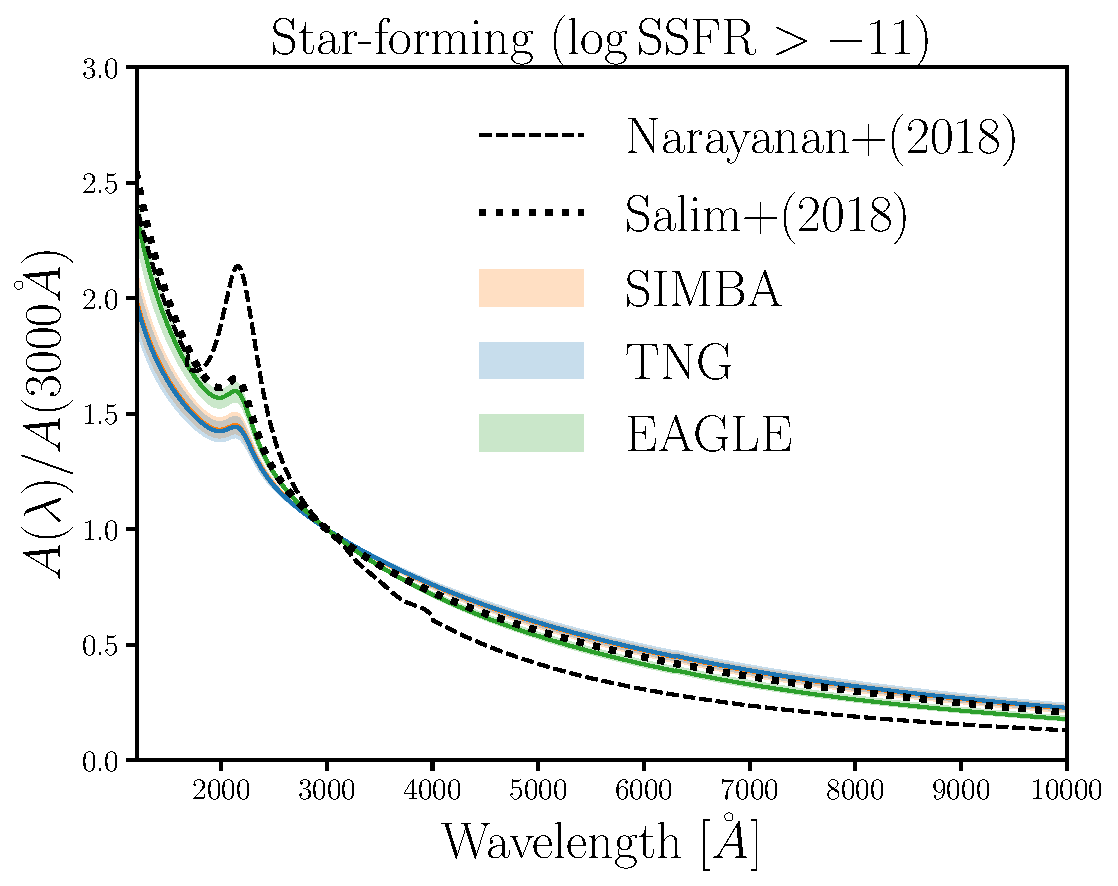
\includegraphics[width=0.5\textwidth]{figs/abc_sf_attenuation.pdf}
    \caption{\label{fig:sfatten}
    \chedit{
        The normalized attenuation curves of star-forming galaxies predicted by
        the \eda~for median posterior parameter values of TNG (blue) and EAGLE
        (green).  
        Galaxies are classified as star-forming using a $\log \ssfr >
        -11~yr^{-1}$ cut. 
        The attenuation curves are normalized at $3000\AA$ and we mark the
        $1\sigma$ standard deviation of the attenuation curves with the shaded
        region.
        For comparison, we include $A(\lambda)/A(3000\AA)$ measurements from
        the\citep{narayanan2018} radiative transfer simulation (dashed) and
        \cite{salim2018} observations (dotted).
        %The \cite{calzetti2000} and \cite{battisti2017} attenuation curves are shallower than the \eda~attenuation curves; however, they probe lower $M_*$ galaxies than our forward modeled TNG and EAGLE samples.  For attenuation curve from \cite{salim2018}, which probe a similar $M_*$ range, we find goood agreement. 
        {\em The \eda~predict attenuation curves of star-forming galaxies that
        are in good agreement with the attenuation curves measured from
        the simulation and observations.}
        %We also find good agreement with median attenuation curve of star-forming galaxies in the radiative transfer simulations of \cite{narayanan2018}.
    }
    }
\end{center}
\end{figure}

\chedit{ 
    In addition to the attenuation-slope relation, we can also directly compare
    the attenuation curves predicted by the \eda~to measurements from
    observations for star-forming galaxies. 
    In Figure~\ref{fig:sfatten}, we present the normalized attenuation curves
    of star-forming galaxies predicted by the \eda~for the median posterior
    parameter values of TNG (blue) and EAGLE (green).
    We define galaxies with $\ssfr > 10^{-11}{yr}^{-1}$ as star-forming.
    The attenuation curves are normalized at $3000\AA$ and we present the
    variation in the attenuation curves in the shaded region, 1$\sigma$
    standard deviation about the median. 
    For comparison, we include $A(\lambda)/A(3000\AA)$ from the
    \cite{narayanan2018} radiative transfer simulation (dashed) and 
    observations~\citep[][; dotted]{salim2018}. 
    The attenuation curve from \cite{salim2018} correspond to star-forming
    galaxies with $M_* > 10^{10.5}M_\odot$, a similar $M_*$ range as our
    forward modeled TNG and EAGLE samples. 
    Since we do not vary the UV bump in our \eda~prescription, we ignore any
    discrepancies in the amplitudes of the bump. 
    \emph{Overall, we find good agreement between the \eda~attenuation curves for
    star-forming galaxies and the attenuation curves from observations and
    simulations.}
}

\chedit{ 
    In this section, we show that \eda~predicts dust attenuation curves that
    are in good agreement with the well-established attenuation-slope relation
    and the attenuation curves of star-forming galaxies from observations and simulations. 
    The \eda~predictions are derived soley from matching the SDSS UV and
    optical color-magnitude relations --- without fitting any observed dust
    attenuation measurements.
    The overall agreement demonstrates the robustness of the \eda~framework and
    the specific parameterization of our \eda~prescription. 
}

%Again, the fact that we reproduce the detailed dust attenuation curves of star-forming galaxies in observations and simulations with the \eda~without fitting for them, highlights the advantages of a forward modeling approach. 

%The \eda~attenuation curves are slightly steeper than the \cite{calzetti2000} and \cite{battisti2017} curves. 
%These attenuation curves, however, are derived from $M_* < 10^{9.9}M_\odot$
%star-forming galaxies, which lie below the $M_*$ limit of our forward
%modeled TNG and EAGLE samples. 
%Meanwhile, the TNG and EAGLE \eda~attenuation curves are in good agreement
%with the \cite{salim2018} attenuation curve for $M_* > 10^{10.5}M_\odot$ star-forming galaxies. 
%They are also consistent with the median curve of \cite{narayanan2018}. 

%The \eda~attenuation curves are noticeably steeper than the \cite{calzetti2000} and \cite{battisti2017} curves.  These attenuation curves, however, are derived from $M_* < 10^{9.9}M_\odot$ star-forming galaxies --- below our $M_*$ range. 
%Since we find $\mdeltam < 0$ for both the TNG and EAGLE posteriors, the \eda~attenuation curves are consistent with \cite{calzetti2000} and \cite{battisti2017}. 


%\chedit{ 
%    The \eda~predicts higher dust attenuation at lower wavelenghts for
%    star-forming galaxies.
%    Without dust attenuation, both TNG and EAGLE predict star-forming galaxies
%    that are bluer in the optical and UV than observations
%    (Figure~\ref{fig:obs}).
%    To reproduce the SDSS, the \eda~significantly reddens star-forming galaxies.
%}
%In Figure~\ref{fig:raw_atten}, we also find that more massive star-forming
%galaxies have higher attenuation. This is because the simulations overpredict 
%luminous blue star-forming galaxies, which must be attenuated to reproduce
%observations. 


%At low attenuation, dust scattering dominates absoprtion so the 
%attenuation curve steepens because red light scatters isotropically while blue light
%scatters forward~\citep{gordon1994, witt2000, draine2003}. %, which causes more optical-to-IR light to escape the galaxy than UV light
%At high attenuation dust absorption is dominant and the attenuation curve is
%shallower~\citep{chevallard2013}. For the $A_V$ range probed by the DEM, the
%$A_V$--slope relation is in good agreement with GSWLC2 galaxies~\citep[black shaded][]{salim2020}.
%They are also consistent with \cite{leja2017}. We also compare our results to
%theoretical predictions from radiative transfer models, \cite{inoue2005}
%(dotted), the radiative transfer models considered in \cite{chevallard2013}
%(dot dashed), and \cite{trayford2020} (light shaded), which all predict shallower 
%attenuation curves than observations. This is also the case for the
%\cite{narayanan2018} attenuation curves (not included). 
%\emph{The attenuation curve slopes from the DEM for are in excellent
%agreement with observations and better reproduces the observed
%attenuation--slope relation than radiative transfer models.}
